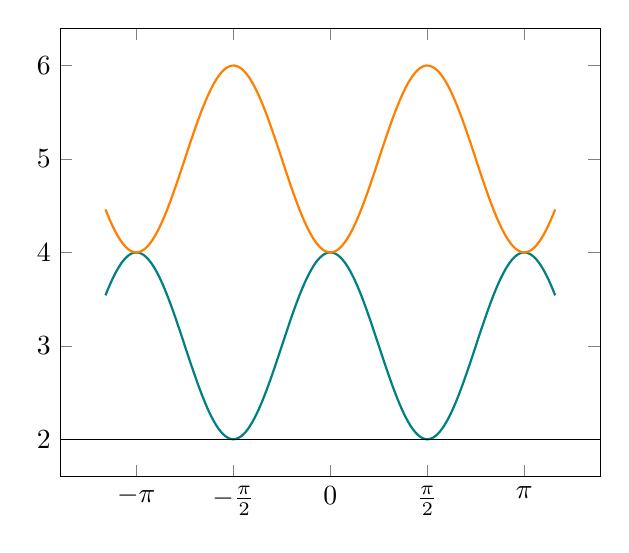
\begin{tikzpicture}
    \begin{axis}[domain=-0.5-pi:0.5+pi,
                 samples = 200,
                 xtick={-3.14159,-1.57089,...,3.14159},
                 xticklabels={$-\pi$,$-\frac \pi 2$,0,$\frac \pi 2$,$\pi$},
                 cycle list name = exotic,
                 legend style={anchor= north west}
                 ]
%    \foreach \q in {0.00,0.05,0.10,0.20,0.50}{
%      \addplot+[mark = none,
%               thick
%               ]
%               {4*\q + 2 + 2*cos(deg(x))^2 + 2*\q*sin(deg(x))^2}; 
%      \addlegendentryexpanded{$q=\q$}
%               }
      \addplot+[
                mark = none,
                thick
               ]
               {2*(1+cos(deg(x))^2)};
      \addplot+[
                mark = none,
                thick
               ]
               {2*(2+sin(deg(x))^2)};
      \draw[] (axis cs:\pgfkeysvalueof{/pgfplots/xmin},2) -- (axis cs:\pgfkeysvalueof{/pgfplots/xmax},2);
    \end{axis}
\end{tikzpicture}
